%%%%%%%%%%%%%%%%%%%%%%%%%%%%%%%%%%%%%%%%%
% Masters/Doctoral Thesis
% LaTeX Template
% Version 2.5 (27/8/17)
%
% This template was downloaded from:
% http://www.LaTeXTemplates.com
%
% Version 2.x major modifications by:
% Vel (vel@latextemplates.com)
%
% This template is based on a template by:
% Steve Gunn (http://users.ecs.soton.ac.uk/srg/softwaretools/document/templates/)
% Sunil Patel (http://www.sunilpatel.co.uk/thesis-template/)
%
% Template license:
% CC BY-NC-SA 3.0 (http://creativecommons.org/licenses/by-nc-sa/3.0/)
%
%%%%%%%%%%%%%%%%%%%%%%%%%%%%%%%%%%%%%%%%%

%----------------------------------------------------------------------------------------
%	PACKAGES AND OTHER DOCUMENT CONFIGURATIONS
%----------------------------------------------------------------------------------------

\documentclass[
11pt, % The default document font size, options: 10pt, 11pt, 12pt
%oneside, % Two side (alternating margins) for binding by default, uncomment to switch to one side
english, % ngerman for German
singlespacing, % Single line spacing, alternatives: onehalfspacing or doublespacing
%draft, % Uncomment to enable draft mode (no pictures, no links, overfull hboxes indicated)
%nolistspacing, % If the document is onehalfspacing or doublespacing, uncomment this to set spacing in lists to single
%liststotoc, % Uncomment to add the list of figures/tables/etc to the table of contents
%toctotoc, % Uncomment to add the main table of contents to the table of contents
%parskip, % Uncomment to add space between paragraphs
%nohyperref, % Uncomment to not load the hyperref package
headsepline, % Uncomment to get a line under the header
%chapterinoneline, % Uncomment to place the chapter title next to the number on one line
%consistentlayout, % Uncomment to change the layout of the declaration, abstract and acknowledgements pages to match the default layout
]{MastersDoctoralThesis} % The class file specifying the document structure

\usepackage[utf8]{inputenc} % Required for inputting international characters
\usepackage[T1]{fontenc} % Output font encoding for international characters

\usepackage{mathpazo} % Use the Palatino font by default

\usepackage[backend=bibtex,style=authoryear,natbib=true]{biblatex} % Use the bibtex backend with the authoryear citation style (which resembles APA)

\addbibresource{namo.bib} % The filename of the bibliography

\usepackage[autostyle=true]{csquotes} % Required to generate language-dependent quotes in the bibliography



%----------------------------------------------------------------------------------------
%	MARGIN SETTINGS
%----------------------------------------------------------------------------------------

\geometry{
	paper=a4paper, % Change to letterpaper for US letter
	inner=2.5cm, % Inner margin
	outer=3.8cm, % Outer margin
	bindingoffset=.5cm, % Binding offset
	top=1.5cm, % Top margin
	bottom=1.5cm, % Bottom margin
	%showframe, % Uncomment to show how the type block is set on the page
}

%----------------------------------------------------------------------------------------
%	THESIS INFORMATION
%----------------------------------------------------------------------------------------

\thesistitle{Toward social navigation among movable obstacles} % Your thesis title, this is used in the title and abstract, print it elsewhere with \ttitle
\supervisor{Dr. Fabrice \textsc{Jumel}\\
			Dr. Jacques \textsc{Saraydaryan}\\
			Dr. Olivier \textsc{Simonin}\\} % Your supervisor's name, this is used in the title page, print it elsewhere with \supname
\examiner{Dr. Jean-François \textsc{Boulicaut}\\
					Dr. Vasile-Marian \textsc{Scuturici}\\
					Dr. Christine \textsc{Solnon}\\} % Your examiner's name, this is not currently used anywhere in the template, print it elsewhere with \examname
\degree{Engineering Degree} % Your degree name, this is used in the title page and abstract, print it elsewhere with \degreename
\author{Benoit \textsc{Renault}} % Your name, this is used in the title page and abstract, print it elsewhere with \authorname
\addresses{} % Your address, this is not currently used anywhere in the template, print it elsewhere with \addressname

\subject{Robotics} % Your subject area, this is not currently used anywhere in the template, print it elsewhere with \subjectname
\keywords{NAMO, Navigation Among Movable Obstacles, Social Navigation} % Keywords for your thesis, this is not currently used anywhere in the template, print it elsewhere with \keywordnames
\keywordsfr{NAMO, Navigation en milieu modifiable, Navigation Sociale}
\university{\href{http://insa-lyon.fr}{National Institute of Applied Sciences of Lyon}} % Your university's name and URL, this is used in the title page and abstract, print it elsewhere with \univname
\department{\href{http://if.insa-lyon.fr}{Computer Sciences and Engineering Department (IF)}} % Your department's name and URL, this is used in the title page and abstract, print it elsewhere with \deptname
\group{\href{https://team.inria.fr/chroma/}{INRIA Chroma team}} % Your research group's name and URL, this is used in the title page, print it elsewhere with \groupname
\faculty{\href{}{}} % Your faculty's name and URL, this is used in the title page and abstract, print it elsewhere with \facname

\AtBeginDocument{
\hypersetup{pdftitle=\ttitle} % Set the PDF's title to your title
\hypersetup{pdfauthor=\authorname} % Set the PDF's author to your name
\hypersetup{pdfkeywords=\keywordnames} % Set the PDF's keywords to your keywords
}

\begin{document}

\frontmatter % Use roman page numbering style (i, ii, iii, iv...) for the pre-content pages

\pagestyle{plain} % Default to the plain heading style until the thesis style is called for the body content

%----------------------------------------------------------------------------------------
%	TITLE PAGE
%----------------------------------------------------------------------------------------

\begin{titlepage}
\begin{center}

\vspace*{.06\textheight}
{\scshape\LARGE \univname\par}\vspace{1.5cm} % University name
\textsc{\Large Research Report}\\[0.5cm] % Thesis type

\HRule \\[0.4cm] % Horizontal line
{\huge \bfseries \ttitle\par}\vspace{0.4cm} % Thesis title
\HRule \\[1.5cm] % Horizontal line

\begin{minipage}[t]{0.4\textwidth}
\begin{flushleft} \large
\emph{Author:}\\
\href{http://littleroot.net/}{\authorname} % Author name
\end{flushleft}
\end{minipage}
\begin{minipage}[t]{0.4\textwidth}
\begin{flushright} \large
\emph{Supervisors:} \\
\supname % Supervisor names
\medskip
\emph{Examiners:} \\
\examname % Examinator names
\end{flushright}
\end{minipage}\\[3cm]

\medskip

\vspace{0.35cm}

\includegraphics[width=5cm]{insa_color.png} % University/department logo - uncomment to place it
\vspace{0.35cm}

\vfill

\large \textit{A report written for the \groupname \\ and submitted in fulfillment of the requirements of the \degreename \\ of the \deptname}\\[0.3cm] % University

\vfill

{\large \today}\\[4cm] % Date

\vfill
\end{center}
\end{titlepage}

%----------------------------------------------------------------------------------------
%	ABSTRACT PAGE
%----------------------------------------------------------------------------------------

\begin{abstract}
\addchaptertocentry{\abstractname} % Add the abstract to the table of contents
\paragraph{Résumé :} Le résumé doit décrire le contenu du rapport. Il doit contenir au moins 70 mots et ne pas dépasser 150 mots. La taille de la police est de 9-point en simple interligne. Il doit y avoir deux lignes vides avant et après le résumé. Ce document est le format exigé pour le rapport de synthèse de PFE.

\paragraph{Mots-clefs :} \keywordnamesfr

\paragraph{Abstract:} The abstract should summarize the contents of the paper and should contain at least 70 and at most 150 words. It should be set in 9-point font size and should be inset 1.0 cm from the right and left margins. There should be two blank (10-point) lines before and after the abstract. This document is in the required format.

\paragraph{Key-words:} \keywordnames
\end{abstract}

%----------------------------------------------------------------------------------------
%	LIST OF CONTENTS/FIGURES/TABLES PAGES
%----------------------------------------------------------------------------------------

%\tableofcontents % Prints the main table of contents

%\listoffigures % Prints the list of figures

%\listoftables % Prints the list of tables

%----------------------------------------------------------------------------------------
%	ABBREVIATIONS
%----------------------------------------------------------------------------------------

% \begin{abbreviations}{ll} % Include a list of abbreviations (a table of two columns)
%
% \textbf{LAH} & \textbf{L}ist \textbf{A}bbreviations \textbf{H}ere\\
% \textbf{WSF} & \textbf{W}hat (it) \textbf{S}tands \textbf{F}or\\
%
% \end{abbreviations}

%----------------------------------------------------------------------------------------
%	PHYSICAL CONSTANTS/OTHER DEFINITIONS
%----------------------------------------------------------------------------------------

% \begin{constants}{lr@{${}={}$}l} % The list of physical constants is a three column table
%
% % The \SI{}{} command is provided by the siunitx package, see its documentation for instructions on how to use it
%
% Speed of Light & $c_{0}$ & \SI{2.99792458e8}{\meter\per\second} (exact)\\
% %Constant Name & $Symbol$ & $Constant Value$ with units\\
%
% \end{constants}

%----------------------------------------------------------------------------------------
%	SYMBOLS
%----------------------------------------------------------------------------------------

% \begin{symbols}{lll} % Include a list of Symbols (a three column table)
%
% $a$ & distance & \si{\meter} \\
% $P$ & power & \si{\watt} (\si{\joule\per\second}) \\
% %Symbol & Name & Unit \\
%
% \addlinespace % Gap to separate the Roman symbols from the Greek
%
% $\omega$ & angular frequency & \si{\radian} \\
%
% \end{symbols}

%----------------------------------------------------------------------------------------
%	DEDICATION
%----------------------------------------------------------------------------------------

% \dedicatory{For/Dedicated to/To my\ldots}

%----------------------------------------------------------------------------------------
%	THESIS CONTENT - CHAPTERS
%----------------------------------------------------------------------------------------

\mainmatter % Begin numeric (1,2,3...) page numbering

\pagestyle{thesis} % Return the page headers back to the "thesis" style

% Include the chapters of the thesis as separate files from the Chapters folder
% Uncomment the lines as you write the chapters

% Chapter 1

\chapter{Introduction} % Main chapter title

\label{Chapter1} % For referencing the chapter elsewhere, use \ref{Chapter1}

% L'introduction situe le problème, l'expose, insiste sur son importance et indique la manière dont il est envisagé. A l'introduction est associée une  présentation préliminaire de la manière de traiter la question (méthode). L'introduction doit aussi exposer l’étude de l’existant dans le domaine précis qui concerne le PFE et faire ressortir la nécessité de réalisations complémentaires comme celle qui fait l'objet du PFE.

\section{Motivation}

\paragraph{} Service robotics are an active research field: there is a growing demand for intelligent machines that are meant to be used in human environments for domestic tasks (e.g, maintaining people homes, entertaining them, caring for them; especially old ones or with disabilities, \dots) \cmmnt{\parencite{mettler_service_2017, graf_care-o-bot_2004}}. To fulfill such tasks, a service robot obviously needs to be able to autonomously navigate through space, according to the given constraints: these navigation capabilities and constraints are the main focus of the following work.

\paragraph{} Human environments represent a very complex challenge, since they are dynamic, alterable and imply social conventions and rules that the robot must also respect in the way it navigates and interacts with the world. For example, in a home setting, humans (or other autonomous actors, such as pets) can be considered as moving obstacles that must be taken into account. Also, for a robot to go from a point A to B, a solution may only be found if it implies moving an obstacle out of the way. And all this must be done in a socially acceptable manner: one would not appreciate a robot moving at high speeds around people or to move obstacles that are not supposed to be moved.

\paragraph{} The most common constraint for robot navigation is solely to find the shortest collision-free path, and this is an acceptable solution in a static context (nothing moves, at the exception of the robot). However, if we want the robot to navigate a human environment, this is not sufficient.

\begin{figure}[H]
\centering
\begin{subfigure}{.48\textwidth}
  \centering
  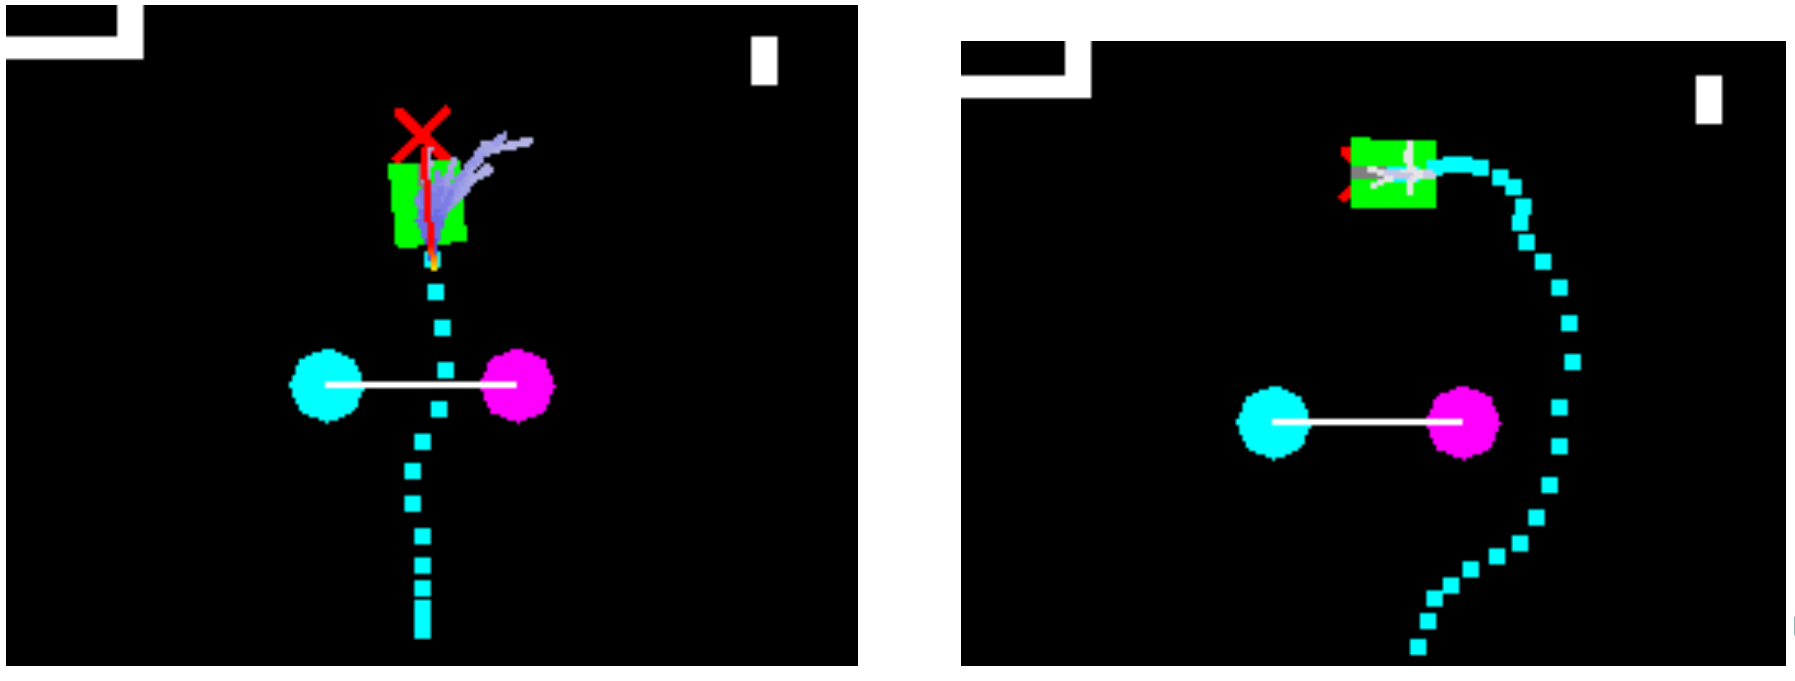
\includegraphics[width=\linewidth]{Figures/Problem_Illustration/social_problem.png}
  \caption{Sample social navigation problem}
  \label{fig:social_problem}
\end{subfigure}\hspace*{\fill}
\begin{subfigure}{.48\textwidth}
  \centering
  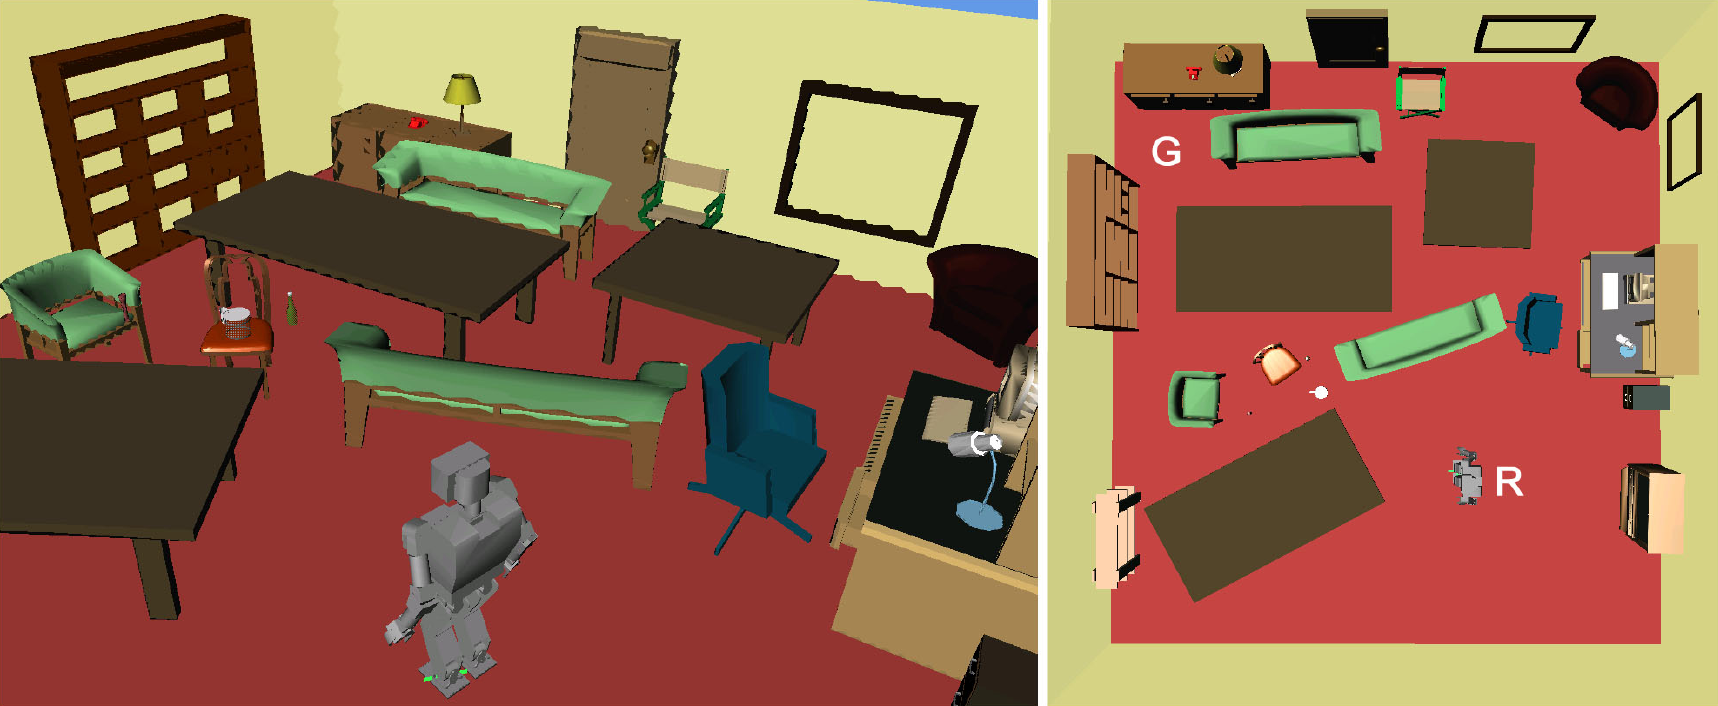
\includegraphics[width=0.9\linewidth]{Figures/Problem_Illustration/namo_problem.png}
  \caption{Sample NAMO problem}
  \label{fig:namo_problem}
\end{subfigure}
\caption{Sample problems for social navigation and NAMO. In the sample social navigation problem, the robot (green square) must reconsider its path to avoid penetrating the zone between the two humans (colored dots) interacting with each other (image from \parencite{rios-martinez_understanding_2011}). In the NAMO problem,  the robot will need to move obstacles in order to access its goal (image from \parencite{stilman_navigation_2005}).}
\label{fig:navigation_problems}
\end{figure}

\paragraph{} To our knowledge, the problem of navigation planning in dynamic environments populated with humans \parencite{kruse_human-aware_2013, rios-martinez_proxemics_2015}, and the problem of navigation planning in robot-alterable environments (which is called Navigation Among Movable Obstacles, or NAMO, more precisely defined in \parencite{stilman_navigation_2007}) have always been treated separately. The \groupname\footnote{Team website: \url{https://team.inria.fr/chroma/}} \, for one, proposed social and dynamic navigation algorithms that optimize the generation of trajectories by managing the risk of colliding with obstacles \parencite{fulgenzi_autonomous_2009, rios-martinez_socially-aware_2013}, respecting social conventions such as avoiding human interaction spaces \parencite{papadakis_adaptive_2014, rios-martinez_understanding_2011} (Figure \ref{fig:social_problem}), or predicting the trajectories of moving obstacles \parencite{jumel_mapping_2017}, \dots The NAMO problem (Figure \ref{fig:namo_problem}) has been dealt with in a great variety of contexts, detailed in Chapter \ref{Chapter2}. It seems that these two problems have yet to be brought together, and the new problematics that are to arise from this confluence are still to be identified and addressed.

\section{Objective}

\paragraph{} The long-term objective behind this work is to allow a real service robot to navigate in complex, human, dynamic and robot-alterable environments, preferably in an optimal way (minimize risk of collision, travel distance, time or energy, \dots).

\paragraph{} More precisely, the context of this long-term objective for formulating, comparing and evaluating hypotheses, is the Robocup@Home\footnote{Competition website: \url{http://www.robocupathome.org/}}. The \groupname \, participates in the standard league of this international-level competition, that provides service robotics challenges to evaluate solutions proposed by researchers and students. The mandatory robotic platform for the standard league is the Pepper robot\footnote{Pepper characteristics are described in Chapter \ref{Chapter5} and also on this website: \url{http://doc.aldebaran.com/2-4/family/pepper_technical/index_dev_pepper.html}}, piloted through ROS\footnote{ROS, the Robot Operating System, website: \url{http://www.ros.org/}} for our team. Notably, this defines the context of our search in that:
\begin{itemize}
  \item only the onboard sensors of the robot are used to update the robot's \textbf{partial environment knowledge} making,
  \item we thus seek \textbf{local optimality}: that is, optimal decision-making given the current belief state of the robot on its environment,
  \item overall, we will privilegiate solutions that are more easily applicable for Pepper. For example, we will prefer a solution that involves pushing rather than grasping obstacles to move them, as Pepper's limited mechanical features make it difficult to grasp obstacles in a safe way for the robot.
\end{itemize}

\paragraph{} In the end, the specific objectives of this first work are to:
\begin{itemize}
  \item explore the NAMO problem domain and extract characteristics that allow to sort through existing works,
  \item identify both new concerns and bridges between this problem and the ones of dynamic and social navigation,
  \item build upon existing work to propose solutions to the previously identified concerns,
  \item and finally validate our propositions in simulation, and as much as possible, in a real setting with the Pepper robot.
\end{itemize}

\clearpage

\section{Overview}

\paragraph{} The following work is organized as follows:

\begin{itemize}
  \item Chapter \ref{Chapter2} is a detailed state of the art of the NAMO domain, and derives comparison criteria from a selection of articles that are closely related to our goals. It also explains the choice of the papers we chose to build upon.
  \item Chapter \ref{Chapter3} is a thorough study and criticism of the chosen base algorithm. We explain the logic of the original algorithm while also providing definitions and conventions that remove the many original ambiguities. Finally, we propose a pseudocode interpretation of the improvements proposed by Levihn et. al. on the first algorithm.
  \item Chapter \ref{Chapter4} revisits the algorithm to really restore optimality, make it stick to our hypotheses, and extend it to solve new social and dynamic environment concerns.
  \item Chapter \ref{Chapter5} recounts our experimentations with the Pepper robot and simulations to validate our propositions.
  \item Chapter \ref{Chapter6} summarizes our contributions and details opportunities for research arisen by this work.
  \item Appendices \ref{algorithms} and \ref{comparison_tables} gather comparison tables and pseudocode representations of algorithm propositions.
\end{itemize}

% Chapter 2

\chapter{Navigation Among Movable Obstacles: state of the art} % Main chapter title

\label{Chapter2} % For referencing the chapter elsewhere, use \ref{Chapter2}

\section{Determining appropriate comparison criteria}

\subsection{Hypotheses}

\subsection{Approaches}

\subsection{Performance criteria}

\begin{figure}[H]
\centering
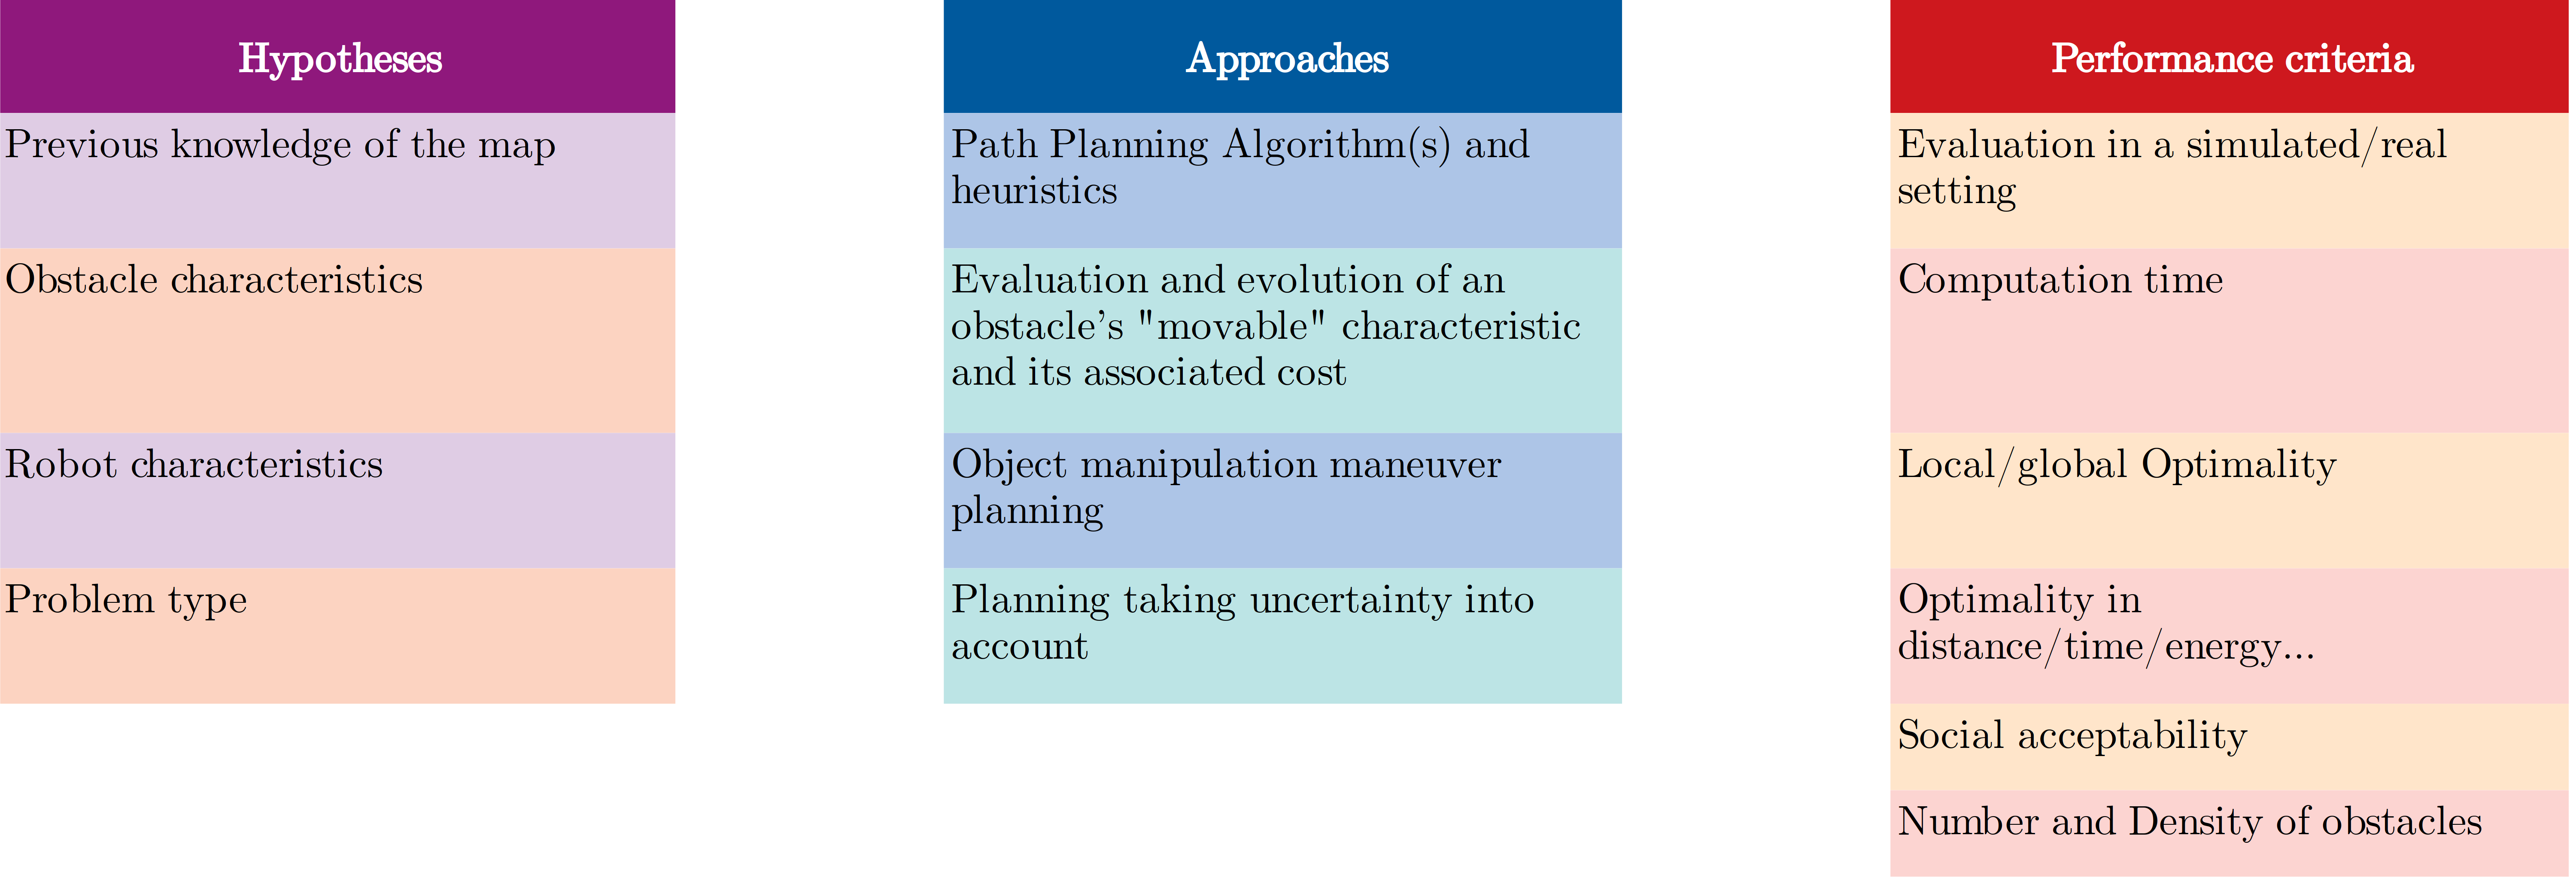
\includegraphics[width=13cm]{Comparison_Table/comparison_criteria}
\decoRule
\caption[Comparison criteria listing]{Comparison criteria, sorted by type: hypotheses, approaches and performance criterias}
\label{fig:comparison_criteria}
\end{figure}

\section{Comparison and cross-comparison}

\subsection{Comparison tables}

\subsection{Conclusions}

\subsection{Situating our work in the established context}

% Chapter 3

\chapter{Study of Wu et. al.'s algorithm for locally optimal NAMO in unknown environments} % Main chapter title

\label{Chapter3} % For referencing the chapter elsewhere, use \ref{Chapter3}

\paragraph{} Given the state of the art presented in the previous chapter and what we aimed to achieve in the available time, we chose to build upon Wu et. al.'s algorithm for locally optimal NAMO in unknown environments.

\section{Original algorithms}

\paragraph{} In Wu et. al.'s proposition, the basic idea is to consider either a plan that doesn't involve interacting with obstacles (which can be achieved with any pre-existing path finding algorithm), or a three-steps plan that consists in, first, reaching the obstacle ($c_{1}$), second, pushing it in a single direction ($c_{2}$), and finally reaching the goal from the position we left the obstacle at ($c_{3}$). This is best shown in figure \ref{fig:Wu_Original_Algorithm-wu_components_illus}.

\begin{figure}[H]
\centering
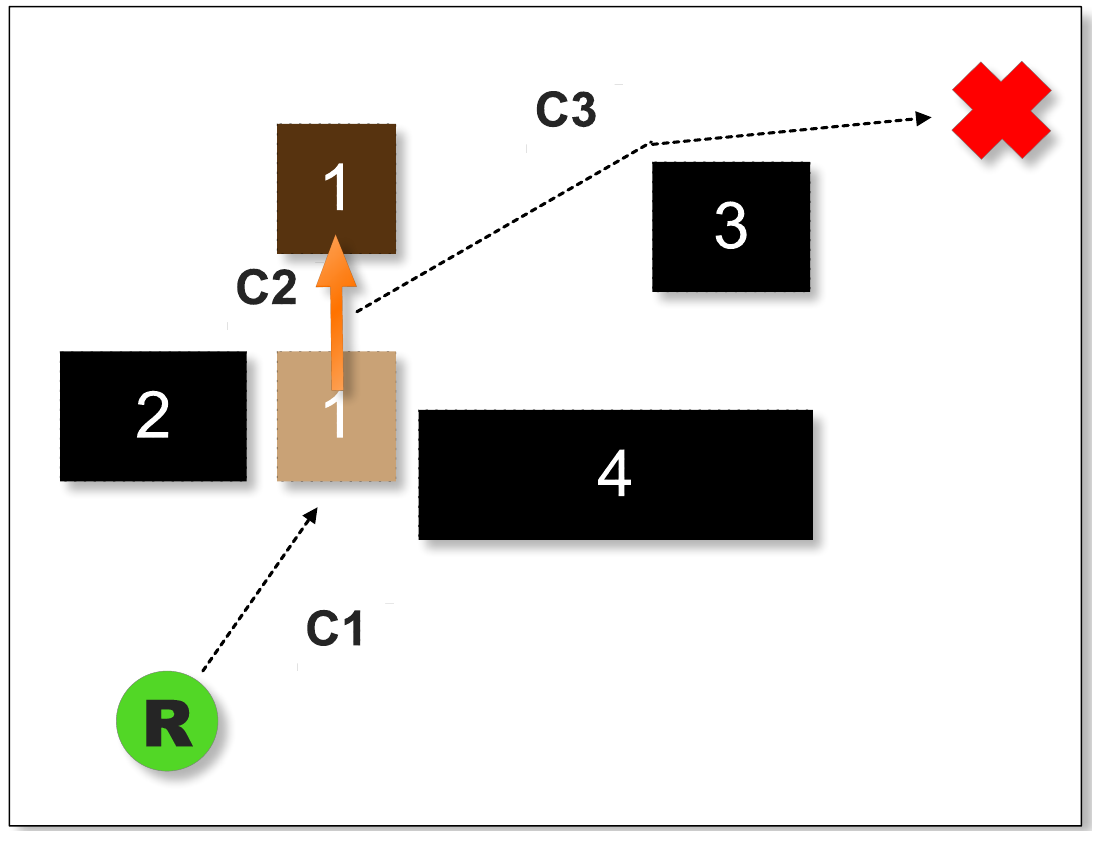
\includegraphics[width=5cm]{Figures/Wu_Original_Algorithm/wu_components_illus.png}
\caption{Figure describing the three plan components when pushing an object, as published in \parencite{wu_navigation_2010}.}
\label{fig:Wu_Original_Algorithm-wu_components_illus}
\end{figure}

\paragraph{} In their first article \parencite{wu_navigation_2010}, Wu et. al. describe two versions of their algorithm: a naive but locally optimal baseline one, and an optimized one, built upon the logic foundation of the first, but that loses its local optimality. In their second article \parencite{levihn_locally_2014}, several other improvements on performance are proposed that restore the local optimality of the proposition. By locally optimal, we mean that the algorithm will \textbf{always} choose the \textbf{best} plan given its current, limited knowledge of the environment.

\paragraph{} The baseline algorithm is very straightforward: it uses an A* path finding subroutine to determine the optimal path between the current robot's position and the goal, avoiding all known obstacles (none at the beginning). As the robot moves forward (Figure \ref{fig:Wu_Original_Algorithm-algo1}, line 17), and therefore gains new information (same figure, line 5), whenever a new obstacle is encountered, every push action for every obstacle is re-simulated (Figure \ref{fig:Wu_Original_Algorithm-algo2}) and compared to the current optimal plan (Figure \ref{fig:Wu_Original_Algorithm-algo1}, line 11). Local optimality is guaranteed for this approach, since the A* algorithm is used with the admissible Euclidean heuristic, thus returning optimal solutions for a given state of the map and goal, and also because whenever a new obstacle is detected (= the map is in a new state), \textbf{all} possible plans are re-evaluated and compared to check if a better plan than the current one can be found or not before moving the robot again.

\begin{figure}[H]
\centering
\begin{subfigure}{.5\textwidth}
  \centering
  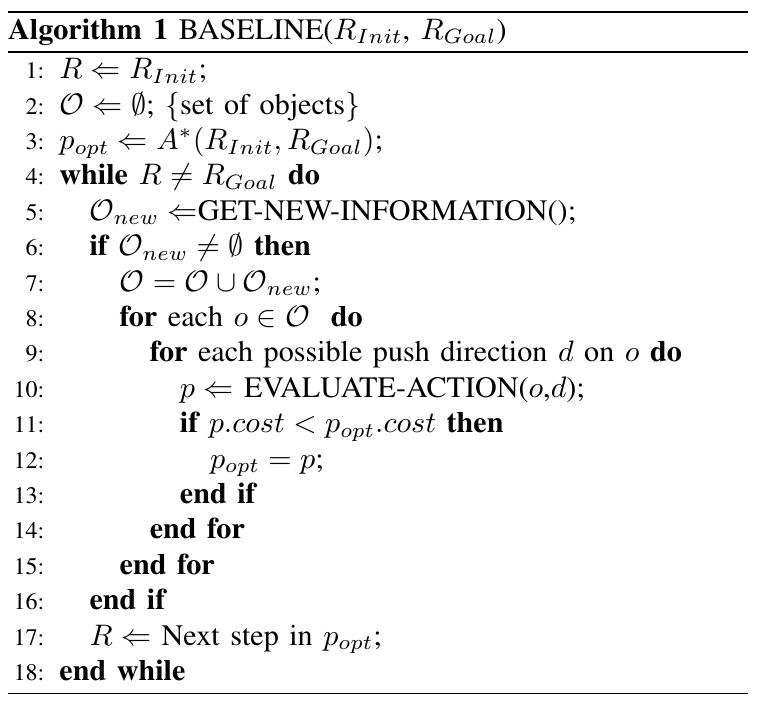
\includegraphics[width=\linewidth]{Figures/Wu_Original_Algorithm/algo1.png}
  \caption{Main loop that evaluates all plans containing the manipulation of an obstacle every time a new one is found}
  \label{fig:Wu_Original_Algorithm-algo1}
\end{subfigure}%
\begin{subfigure}{.5\textwidth}
  \centering
  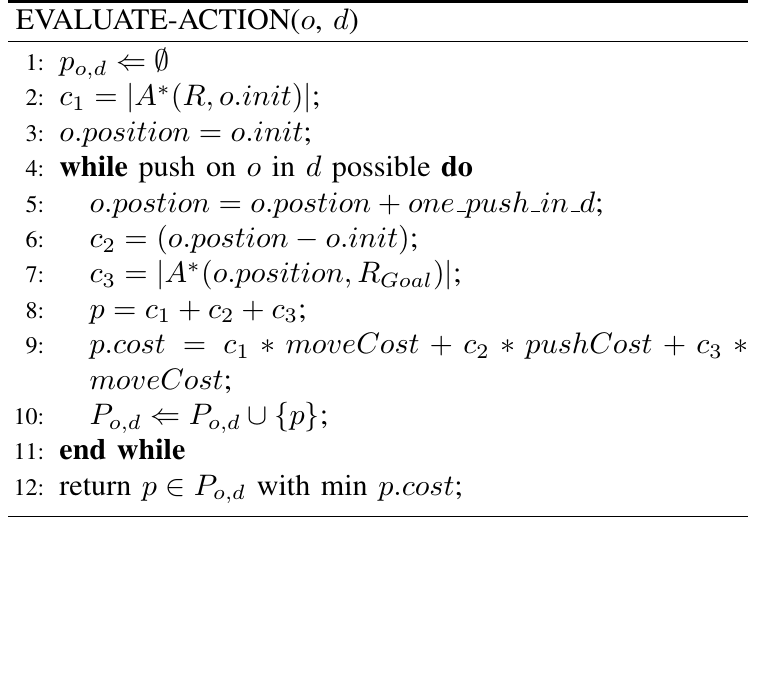
\includegraphics[width=\linewidth]{Figures/Wu_Original_Algorithm/algo2.png}
  \caption{Subroutine for evaluating all possible plans for each manipulation direction allowed on an obstacle}
  \label{fig:Wu_Original_Algorithm-algo2}
\end{subfigure}
\caption{Baseline Algorithm as published by Wu et. al. in \parencite{wu_navigation_2010}}
\label{fig:Wu_Original_Algorithm-baseline}
\end{figure}

\paragraph{} The optimized version of the algorithm published in the first article offers four optimization steps:

\paragraph{First Optimization}\label{optimization_1} Only consider computing a new plan if the current one is actually blocked by a new obstacle (Figure \ref{fig:Wu_Original_Algorithm-algo3}, line 6). This keeps the local optimality, since a newly detected obstacle can only imply a costlier plan either moving around it or moving it (\textbf{assuming obstacles don't move by themselves, which could open new, better routes}): given that we can assume that our current optimal plan was optimal before the discovery of the new obstacle, we need only reconsider it if the new obstacle actually prevents it from coming to fruition.

\paragraph{Second Optimization}\label{optimization_2} Stop simulating pushes in a given direction before it becomes costlier than the current valid optimal plan, thanks to a bound (Figure \ref{fig:Wu_Original_Algorithm-algo4}, line 5). This also keeps optimality, since there are no reasons to continue evaluating actions that are already costlier than simply following the current valid optimal plan.

\paragraph{Third Optimization}\label{optimization_3} Only compute the third path component (from obstacle to goal) with A* if the simulated movement actually creates an opening (Figure \ref{fig:Wu_Original_Algorithm-algo4}, line 7), since checking an opening creation is less computing time-consuming than running a search algorithm to the goal. However, this step also causes the loss of local optimality, because it prevents the algorithm to fully evaluate some plans that could improve the cost. Below are examples figures of cases where this happens, assuming the cost of following a path is the same whether it implies moving an obstacle or not. In Figure \ref{fig:corridor_case} and \ref{fig:openspace_case}, no new opening is ever found, either because the blocking areas around the obstacle don't change (\ref{fig:corridor_case}) or because there were no blocking areas to begin with (\ref{fig:openspace_case}). Theses case are tentatively adressed in Chapter \ref{Chapter4}.

\begin{figure}[H]
\centering
\begin{subfigure}{.5\textwidth}
  \centering
  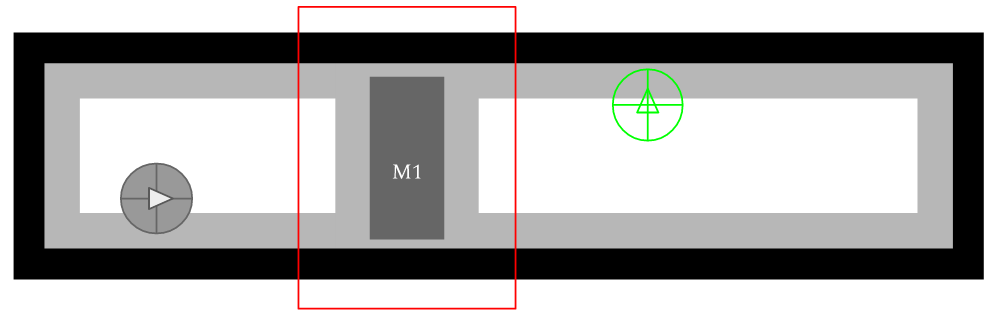
\includegraphics[width=\linewidth]{Figures/Check_New_Opening/corridor_original.png}
  \caption{Initial situation.}
  \label{fig:corridor_original}
\end{subfigure}%
\begin{subfigure}{.5\textwidth}
  \centering
  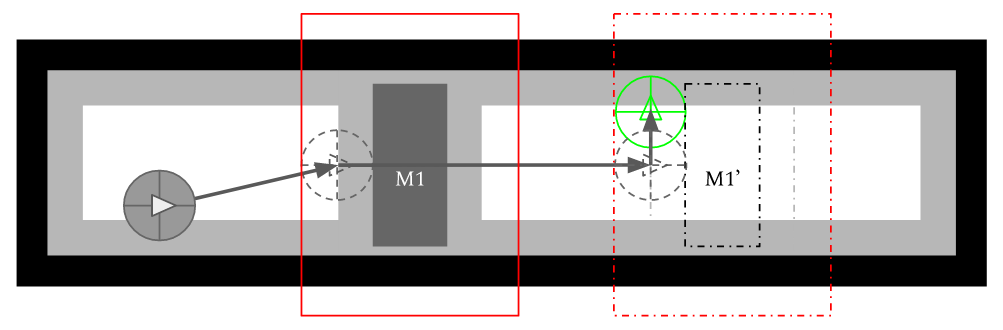
\includegraphics[width=\linewidth]{Figures/Check_New_Opening/corridor_optimal_path.png}
  \caption{Expected plan.}
  \label{fig:corridor_optimal_path}
\end{subfigure}
\caption{"Corridor" case where the original algorithm will not even find a plan when it should.}
\label{fig:corridor_case}
\end{figure}

\begin{figure}[H]
\centering
\begin{subfigure}{.45\textwidth}
  \centering
  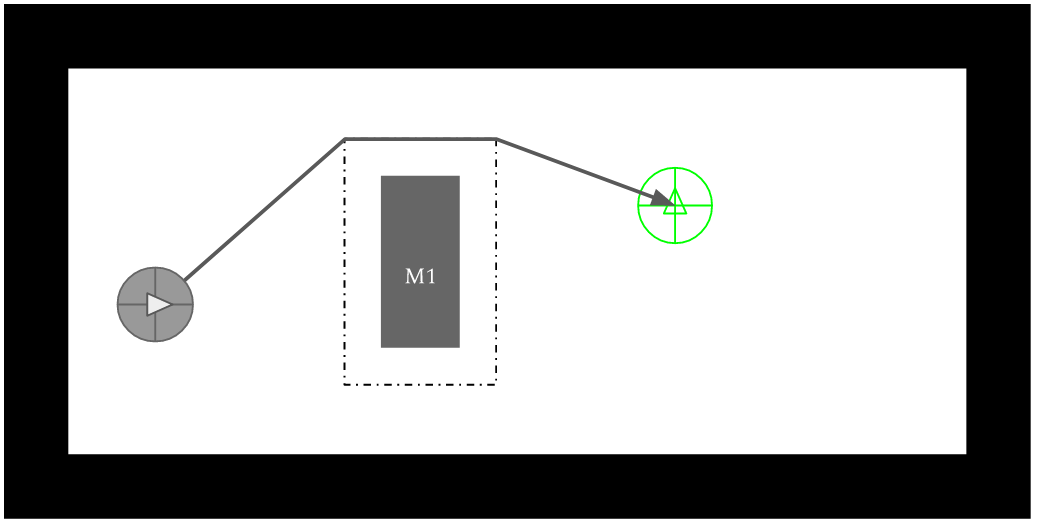
\includegraphics[width=\linewidth]{Figures/Check_New_Opening/openspace_original.png}
  \caption{Initial situation and suboptimal plan avoiding the obstacle that will be returned by the original algorithm.}
  \label{fig:openspace_original}
\end{subfigure}%
\begin{subfigure}{.45\textwidth}
  \centering
  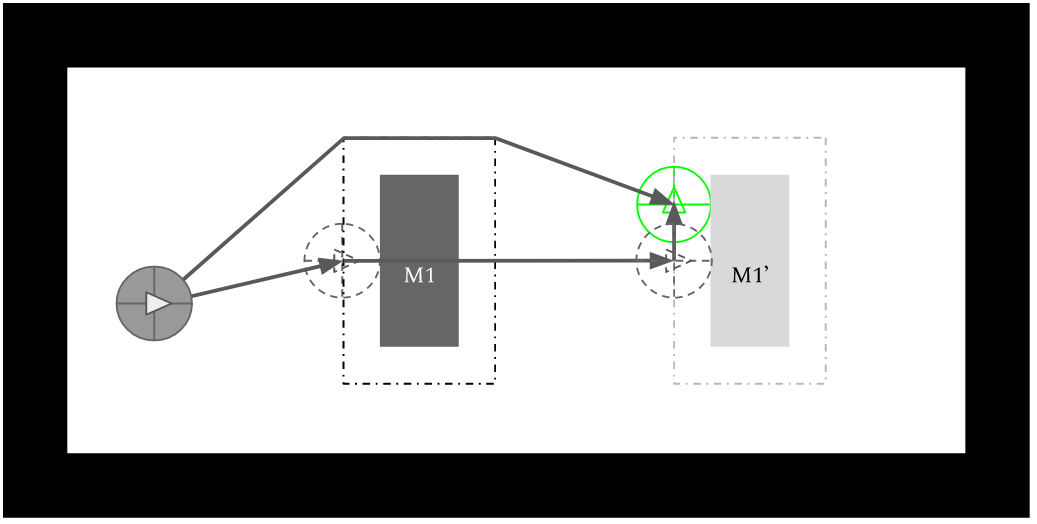
\includegraphics[width=\linewidth]{Figures/Check_New_Opening/openspace_optimal_path.png}
  \caption{Expected plan is the one that pushes the obstacle.}
  \label{fig:openspace_optimal_path}
\end{subfigure}
\caption{"Open space" case where the original algorithm will find only a suboptimal plan.}
\label{fig:openspace_case}
\end{figure}

\paragraph{Fourth Optimization}\label{optimization_4} Finally, when the plan needs to be re-evaluated, new obstacles are evaluated first(Figure \ref{fig:Wu_Original_Algorithm-algo3}, lines 8 to 12) and the resulting paths are saved into a list (Figure \ref{fig:Wu_Original_Algorithm-algo3}, lines 2 and 10) by growing order of an underestimated heuristic cost that corresponds to sum of the costs of the plan components $c_{2}$ and $c_{3}$ (Figure \ref{fig:Wu_Original_Algorithm-algo4}, line 12). Then, this list is used to iterate over all obstacle/push direction combinations, and re-evaluate the corresponding plan (Figure \ref{fig:Wu_Original_Algorithm-algo3}, lines 13 to 20). The re-evaluation can be stopped as soon as the next pair to consider has a heuristic cost greater than the cost of the current optimal plan, improving execution performance (Figure \ref{fig:Wu_Original_Algorithm-algo4}, line 14). However, this optimization step causes the loss of the guarantee of optimality. The heuristic cost depends on $c_{2}$ and $c_{3}$, and when moving an obstacle, these components' costs may get lower. As the algorithm never updates the heuristic cost ($minCost$) in the list according to this possibility, there is therefore no guarantee that the heuristic cost will always be an underestimate. In the words of Levihn, main author of the second article:  \textit{"Second, as the algorithm does not acknowledge the fact that free-space can be created during the execution (e.g. by moving objects), which can lower c2 or c3 for some objects, this optimization steps sacrifices local optimality."} \parencite{levihn_locally_2014}

\paragraph{Note on the use of A* in the main loop} In Figure \ref{fig:Wu_Original_Algorithm-algo3}, lines 3 and 7, a call to the A* algorithm is made. For line 3, it determines the optimal path from the initial position to the goal, supposing no obstacle has been detected yet. In line 7, after the current optimal path has been invalidated by the detection of a collision between this path and a new obstacle, this call to A* star allows to get a new optimal path that avoids all obstacles that will serve as basis for the comparison with paths that consider moving obstacles.

\begin{figure}[H]
\centering
\begin{subfigure}{.45\textwidth}
  \centering
  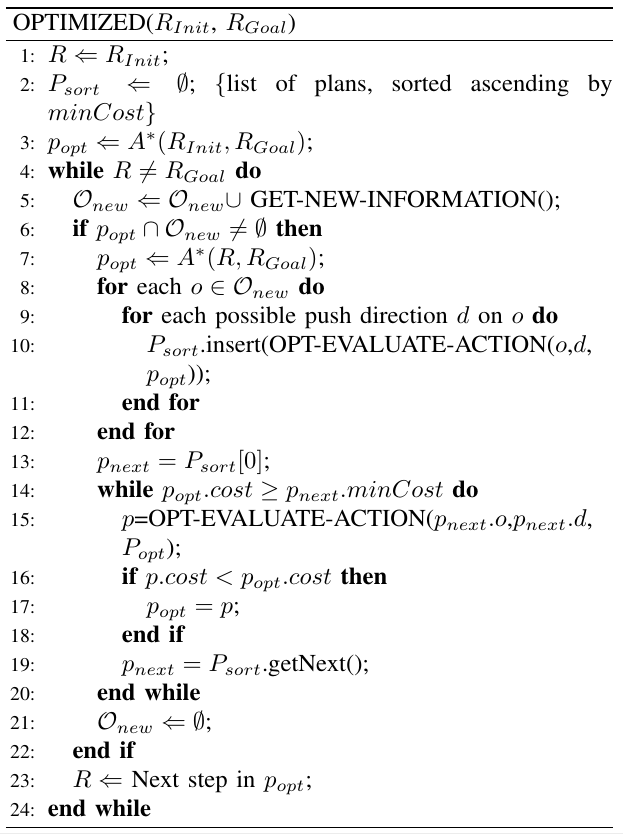
\includegraphics[width=\linewidth]{Figures/Wu_Original_Algorithm/algo3.png}
  \caption{Main loop}
  \label{fig:Wu_Original_Algorithm-algo3}
\end{subfigure}%
\begin{subfigure}{.45\textwidth}
  \centering
  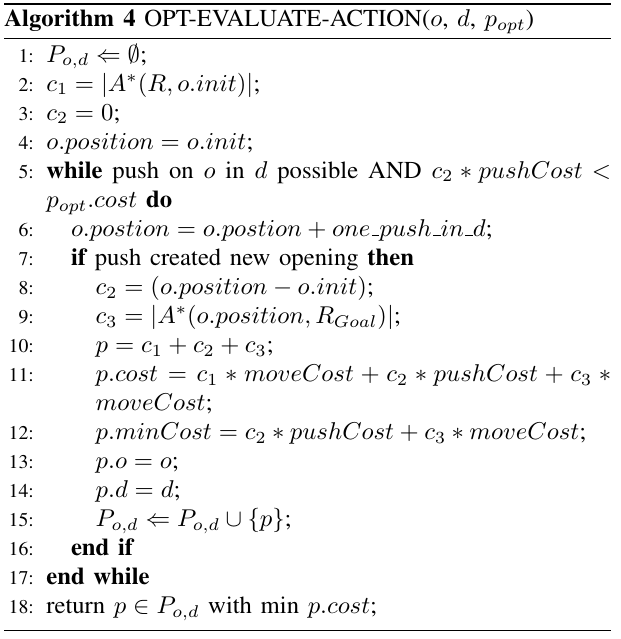
\includegraphics[width=\linewidth]{Figures/Wu_Original_Algorithm/algo4.png}
  \caption{Subroutine}
  \label{fig:Wu_Original_Algorithm-algo4}
\end{subfigure}
\caption{Optimized Algorithm as published by Wu et. al. in \parencite{wu_navigation_2010}}
\label{fig:Wu_Original_Algorithm-optimized}
\end{figure}

\section{Removing ambiguity}\label{removing_ambiguity_section}
\paragraph{} The original pseudocode presented above has quite a few typos, implicit or incongruous notations that create ambiguity (e.g., storing costs and paths in the same variable, having two different variable affectation operators ($\gets$ and $=$), ...), confusing the reading. Since no pseudocode is provided by the authors for the second article's improvements propositions, it was necessary to first fix the pseudocode of the first article. The following paragraphs and the pseudocode formulation \ref{appendix_reworked_wu_section} in Appendix \ref{algorithms} aim at fixing this.

\paragraph{A foreword on notations:}

\begin{itemize}
  \item Paths are ordered sets of "steps", which are themselves robot poses.
  \item Calling the A* or D*Lite algorithms returns A PATH. If no path is found, the returned set is empty: $\emptyset$.
  \item Plans are to be noted with a lowercase $p$. Lists or sets of plans will be noted with an uppercase $P$. A plan is a data structure with a "components" list attribute in which paths are stored in order of execution, and a "cost" attribute that represents the cost of executing the plan.
  \item Components of a plan are noted with a lowercase $c$.
  \item Assuming we suppose a cost in distance, the norm of a path $path$ (written $|path|$) corresponds to the sum of the euclidean distances between consecutive steps, and $+\infty$ if the path is empty.
  \item $moveCost$ and $pushCost$ are constants without dimension.
  \item The current robot pose is to be noted with an uppercase $R$, the initial pose with $R_{init}$ and the goal pose with $R_{goal}$
  \item Obstacles are to be noted with a lowercase $o$. Lists or sets of obstacles will be noted with an uppercase $O$.
\end{itemize}

\paragraph{Note on update}\label{update-from-new-information_note} In the original paper, it is not explicit how the GET-NEW-INFORMATION method works. We therefore changed it to UPDATE-FROM-NEW-INFORMATION() method, that updates the world representation $I$ given in parameter, with new information about obstacles that is collected in parallel in a different execution thread. By that we mean, if this new information includes modifications to known obstacles, they are updated, and if there are new obstacles, they are added to $I$. We assume that the attribute $I$.occGrid corresponds to the occupation grid with inflated obstacles in the current state, so that the path finding routine may run with it. In the same way, $I$.newObstacles corresponds to the list of newly observed obstacles since the last call of the same method.

\paragraph{Note on intersection detection}\label{intersection_note} The $p_{opt} \bigcap \mathcal{O}_{new} \neq \emptyset$ notation is used here as shorthand for checking that any of the new obstacles do not intersect with the robot's path. In implementation, this could be done for example by checking whether every pose in the path is not comprised in the inflated obstacles representation.

\paragraph{Note on re-evaluation}\label{re-evaluation_note} The way the algorithm is written now, even new obstacles that have just been evaluated might be reevaluated, since they have been inserted into the $P_{sort}$ list right before. Consequently, we should add a condition $p_{next}.o \notin \mathcal{O}_{new}$ around the line \ref{lst:line:suppcondition} of Algorithm \ref{alg:01-wu-optimized-part1} to further optimize the algorithm.

\paragraph{Note on getNext}\label{getnext_note} This is a helper method to traverse a list. It returns null when all elements have been traversed.

\paragraph{Note on stop condition}\label{stop_condition_note} The algorithm's stop condition is not explicit in none of the articles. If no path has been found even after considering all relevant obstacles, then the algorithm must return a success value.

\paragraph{Note on plan following}\label{plan_following_note} In the article, the hypothesis is given that if the robot tries to move an obstacle but does not succeed, this obstacle will never be considered for manipulation again. It is meant to allow the robot to detect unmovable obstacles and to avoid an infinite loop caused by an endless evaluation of a same obstacle that cannot be moved. This hypothesis is translated in pseudocode by replacing the vague "$R \gets$ Next step in $p_{opt}$" statement by checking whether the robot actually checking whether robot succeeded or not the desired movement by comparing the actual pose $R_{real}$ after execution and the one we wished to reach $R_{next}$ , and using the $blockedObsL$ set to remember obstacles that should never be evaluated again.

\paragraph{Note on obstacle push pose}\label{obstacle_pushpose_note} For a given obstacle, the algorithm iterates over every push direction applicable to it, but doesn't iterate over every point from which it could apply said push direction. We must deduce that there is an \textbf{implicit hypothesis that for a given push direction, only one point around the obstacle is a valid manipulation start point}. Therefore, we will assume that $o.init$ corresponds to the pose the robot must get into in order to move obstacle $o$ in direction $d$. From the video\footnote{\url{https://youtu.be/oQZLbJHYrl8}} that presents an implementation of the original algorithm, this pose:

\begin{itemize}
  \item Is orientated in the given direction, toward the side of the obstacle that allows to push in the given direction,
  \item Is situated on precomputed "manipulation points" that are at a robot radius distance from the side; often it seems that this point is in front of the side's middle point,
  \item Among these "manipulation points" it seems the one closest to the current position of the robot is chosen. This is fine since the algorithm seems to operate under the \textbf{implicit hypotheses that the friction between the ground and the obstacle is negligible, and that the robot's width is always smaller than the length of the obstacle's side being pushed}. Thus, if the obstacle is movable and not blocked by surrounding obstacles, it will move in the direction it is being pushed in, whatever the accessible "manipulation point" on the appropriate side may be.
\end{itemize}

\paragraph{Note on $c_{1} \neq \emptyset$}\label{c1_note} This condition is not in the original pseudocode, but is necessary to avoid the limit case where no path from the current robot pose to the obstacle is found, in which case, the manipulation plan cannot exist.

\paragraph{Note on bounding}\label{bound_note} It is not said in the article how the "push on $o$ in $d$ possible" condition is verified, but we can assume that it is checked by verifying at each step that the obstacle's new occupied space doesn't intersect with any other obstacle. The $c_{2} * pushCost$ bound here is not tight at all, which is fixed in the new optimization steps proposed in the second article. Still, it allows to cut down on unnecessary evaluations of extra pushes.

\paragraph{Note on $I.withSimulatedObstacleMove$}\label{i_note} This notation is to explicit the fact that the $c_{3}$ component must be computed assuming that the obstacle has been pushed, otherwise it does not make any sense.

\paragraph{Note on elementary push}\label{push_in_d_note} It is not explicit in the article how an elementary $one\_push\_in\_d$ is computed, but we can assume it is the multiplication of a distance constant by the unit direction vector for the given direction $d$. We will make this more explicit in our own algorithm.

\paragraph{Note on opening detection}\label{opening_detection_note} Opening detection is not adressed in this paper and the method used is not explicit. A technical paper later written by co-authors Levihn and Stilman \parencite{levihn_efficient_2011} however clears this ambiguity: \textit{"The algorithm did not rely on search but simply observed the amount of adjacent free spaces on corners of the manipulated obstacle. While efficient, this algorithm is only applicable for world configurations populated with simple rectangular shaped static and movable obstacles. This is not realistic."}.

\paragraph{Note on $c_{2}$}\label{c2_note} As we only admit pushes in straight lines, and because the previous "push on $o$ in $d$ possible" condition means that there will be no collision on the manipulation path, $c_{2}$ simply is a path made from the pose to start moving the object and the pose where the robot leaves it.

\paragraph{Note on $c_{3} \neq \emptyset$}\label{c3_note} This condition is not in the original pseudocode, but is necessary to avoid the limit case where no path from the obstacle to the goal is found, in which case, the manipulation plan cannot exist.

\section{Pseudocode expression of Levihn's recommendations}

\label{levihn_pseudocode_section}

\paragraph{} In the second article \parencite{levihn_locally_2014}, Levihn brings alternate solutions for the \nameref{optimization_2}, \nameref{optimization_3} and \nameref{optimization_4}, reducing the computational effort and enlarging the scope of problems the algorithm can manage. For the \nameref{optimization_4}, the changes make it so optimality is not affected by this optimization step. Our pseudocode formulation \ref{appendix_levihn_interpretation_section} is available in Appendix \ref{algorithms}.

\paragraph{\nameref{optimization_2}} In this article, the authors precise that they are using an improved opening detection algorithm, detailed in their separate technical paper \parencite{levihn_efficient_2011}. Since contrary to the previous one, this new algorithm doesn't rely on obstacles being rectangles, but accepts any kind of polygon, it extends the capability of the overall algorithm to any convex polygon.

\paragraph{} \textbf{However, in the same way we proved that using opening detection for considering the computation of a full plan affected optimality before, since no measures are proposed in this new article to take this into account, we must assume that local optimality is not restored}. In Chapter \ref{Chapter4}, \hyperref[check_opening_solution]{we propose a measure for restoring optimality}.

\paragraph{\nameref{optimization_3}} The bound that allows to reduce the number of unnecessary evaluations of extra pushes is tightened by adding to the current value of $|c_{2}|$ the cost of the first plan component $c_{1}$ and an underestimate of the cost of the third plan component $c_{3}$. This underestimate is the euclidean distance between the last position of the simulated push pose $oSimPose$ and the goal pose $R_{goal}$. This bound is thus proved to be an underestimate of the real cost, keeping optimality.

\paragraph{\nameref{optimization_4}} Last but not least, a new heuristic is proposed alongside a modified version of the previous one. Basically, all obstacles that haven't been evaluated at least once are ordered in a separate list $euCostL$ by a heuristic cost that is independent from $c_{2}$ and $c_{3}$: the euclidean distance between the goal pose $R_{goal}$ and the obstacle's nearest "manipulation point" at which the robot could manipulate it. When an obstacle has been evaluated, it is added to another list $minCostL$ ordered by the usual $minCost$. Since this heuristic is more informed, $minCostL$ is used first when available. If not, $euCostL$ is used, the obstacle is re-evaluated and naturally added to the list ordered by $minCost$. This is achieved through the use of separate indexes for traversing the lists: $i_{e}$ and $i_{m}$. This heuristic is invalidated anytime an obstacle has changed of place, potentially lowering $c_{2}$ or $c_{3}$. Thus, local optimality is no longer affected. For a more detailed explanation, please consult the following pseudocode or the original article \parencite{levihn_locally_2014}.

\paragraph{Reordering the algorithm} Since this is an interpretation, and for easier understanding, we took the liberty of cutting the "OPTIMIZED" algorithm (main loop) into two algorithms: the main loop where the plan is executed and knowledge about the environment updated (i.e. Algorithm \ref{alg:02-levihn-makeandexecuteplan}: "MAKE-AND-EXECUTE-PLAN"), and the subroutine where the iteration over the obstacles is done to generate a new plan when necessary (i.e Algorithm \ref{alg:02-levihn-makeplan}: "MAKE-PLAN"). We also renamed the "OPT-EVALUATE-ACTION" subroutine (i.e Algorithm \ref{alg:01-wu-optevaluateaction}) into "PLAN-FOR-OBSTACLE" (i.e Algorithm \ref{alg:02-levihn-planforobstacle}). Note that the parameters $p_{opt}$, $euCostL$ and $minCostL$ are directly modified during the execution of the MAKE-PLAN() method, hence no return statement in it.

\paragraph{Note on D*Lite}\label{d_star_note} In the second article, it is mentionned twice that the path finding subroutine has been changed from A* to D*Lite. However, not even a hint of an explanation is given as to why this change, or what difference in the implementation it makes. Therefore, in our later final implementation, we shall stick with A*.

\paragraph{Note on update}\label{second_update-from-new-information_note} In addition to the previous note (\ref{update-from-new-information_note}) We assume that $I$.freeSpaceCreated is True if any obstacle's occupied space has been reduced, False otherwise, and that $I$.allObstacles is the list of all observed obstacles in the current state.

\paragraph{Note on getting the list element and limit cases}\label{get_list_element_note} For the sake of readability in the pseudocode, if the list element that is asked for is out of bounds (empty list or reached end of list), the "[ ]" operator shall return a "fake" tuple with a null obstacle reference, and infinite cost: \{null, $+\infty$\}. This could easily be implented in code by either using a ternary operator (for example, "$minCostL[i_{m}].minCost$" would become "$minCostL[i_{m}] =$ null ? $+\infty: minCostL[i_{m}].minCost$") or implementing a custom array object with the wanted behaviour.

\paragraph{Note on $evaluatedObstacles$}\label{evaluated_obstacles_note} $evaluatedObstacles$ is a set that remembers which obstacles have been evaluated in the current MAKE-PLAN instance. This is not mentioned in the original article, but it avoids evaluating an obstacle twice when it is added to $minCostL$.

\paragraph{Traversal note}\label{list_traversal_note} Stop condition: if the next entry from $minCostL$ or $euCostL$ to be considered (the one with the lowest cost) is associated with a cost that is greater than the current optimal plan, it is not worth trying to evaluate any more options, and therefore the loop must end.

\paragraph{Note on priority}\label{minCostL_priority_note} If the current lowest cost entry is minCostL, evaluate the associated obstacle.

\paragraph{Note on postponing}\label{postponing_note} If $i_{e}$ points to a lower cost than the one pointed by $i_{m}$, we only evaluate the associated object if $minCostL$ doesn't already contain an evaluation for it (because there is tighter bound for the cost of moving the object): the evaluation is thus postponed until the obstacle is reached through $minCostL$.

\paragraph{Note on manipulation points \& $c_{1}$'s computation}\label{c1_computation_note} In the article, the authors claim that \textit{"c1 only needs to be calculated once for the entire process of evaluating the current object."}. With the same reasoning as in \nameref{obstacle_pushpose_note}, this affirmation can only be true if the algorithm operates under the \textbf{implicit hypothesis that for all given manipulation directions, only one point around the obstacle is considered a valid manipulation start point}. From \href{https://youtu.be/3AvfPVzBb-s}{the video} accompanying the article, this point seems to be the nearest point from the robot, situated at a radius distance from the middle of a side of the obstacle. However, this hypothesis actually hinders optimality: if there is in fact a valid manipulation point for each side of the obstacle, and the algorithm knowingly doesn't consider them because they are further from the current robot's position, it will ignore the fact that a same manipulation direction could end up in opening a better path if the obstacle were moved from another manipulation point (see figures below). To guarantee optimality, we would have to simulate the manipulation in the given direction for every reachable manipulation point, thus re-evaluating $c_{1}$ for each. That would result in adding an extra "for" loop englobing the existing one. This is illustrated by the figures below.

\begin{figure}[H]
\centering
\begin{subfigure}{.5\textwidth}
  \centering
  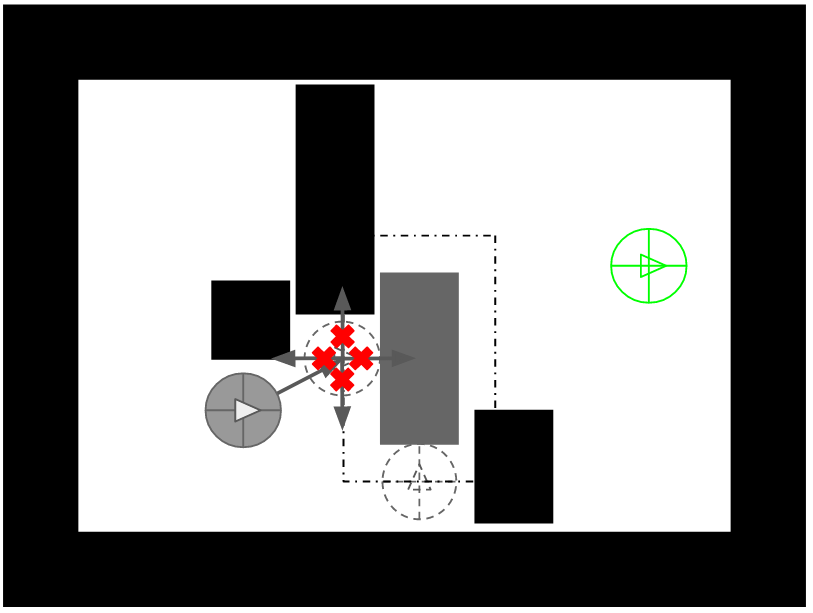
\includegraphics[width=\linewidth]{Figures/Manipulation_Pose/manip_pose_1.png}
  \caption{Nearest manipulation pose doesn't allow moving the obstacle at all.}
  \label{fig:manip_pose_1}
\end{subfigure}%
\begin{subfigure}{.5\textwidth}
  \centering
  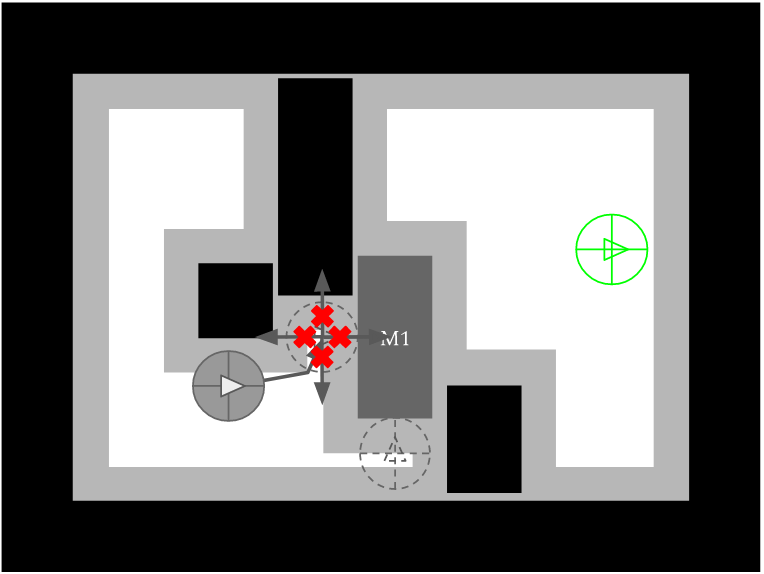
\includegraphics[width=\linewidth]{Figures/Manipulation_Pose/manip_pose_2.png}
  \caption{But if we also consider the other pose, a valid plan can be found.}
  \label{fig:manip_pose_2}
\end{subfigure}
\caption{Illustration of the importance of considering all possibles manipulations for all manipulation poses and not just considering the nearest one.}
\label{fig:manipulation_poses}
\end{figure}

\paragraph{Note on BA}\label{remember_ba_note} The BA variable in the OPT-EVALUATE-ACTION() function allows to remember the initial blocking areas when using the new algorithm for more efficient opening detection. On the first called, the variable is initialized with the initial blocking areas, and at each following call, it is passed as a parameter to reduce computational overhead. This measure is recommended by the technical paper.

\paragraph{Note on allowed manipulations}\label{allowed_manipulations_note} In the second article, the authors assert that they don't limit manipulation to pushes. However, it is clear, especially from \href{https://youtu.be/3AvfPVzBb-s}{the video}, that manipulations are restricted to translations in a single direction.

\paragraph{Note on $seq$}\label{seq_note} Seq corresponds to the number of unit translations that have been simulated.

% Chapter 4

\chapter{Extension of Wu et. al.'s algorithm toward social and dynamic navigation} % Main chapter title

\label{Chapter4} % For referencing the chapter elsewhere, use \ref{Chapter4}

\section{Discussion on the original hypotheses in the light of tests with the Pepper robot}\label{discussion_hypotheses_section}

\paragraph{} The pseudocode formulation \ref{appendix_basicmods_section} for this proposition is available in Appendix \ref{algorithms}.

\paragraph{} As eventually our experimental platform is to be a Pepper robot in the context of the Robocup@Home challenge that emulates a home setting, several hypotheses from the original algorithms have to be reconsidered:

\begin{itemize}
  \item \textbf{Initial knowledge of the environment} is partial, in that all static obstacles (i.e. objects that are not meant to be moved by any actor, like walls or very heavy furniture) have already been mapped. In the context of the Robocup@Home Challenge, participants are allowed to build such a map prior to the actual trials. This hypothesis is actually quite justified since in a home setting, it is very likely that the robot has undergone a configuration phase prior to its daily use, when it is provided with a manually drawn map of the home, or at least allowed to roam about and map the static obstacles. Having a map of static obstacles is very important for standard localization algorithms used in ROS, like \href{http://wiki.ros.org/amcl}{AMCL}, since they use this environment knowledge to compensate for odometry error.
  \item \textbf{Manipulation actions}, for the moment, are to be limited to pushes in a perpendicular direction to the obstacle's side being pushed. Given the many problematics related to grasping objects (e.g., appropriate positioning of the robot joints, keeping the robot balanced, ...), it is best for a first iteration not to dwell on these.
  \item \textbf{Manipulation poses} are a key concept of manipulating obstacles, as we have shown in the previous chapter, and, contrary to the original algorithms we will explicitly explain our hypotheses as to them. Experimentations with the Pepper Robot (see Chapter \ref{Chapter5}) and carboard boxes as movable obstacles have shown that a good first approximation that guarantees quasi-systematic push manipulation successes are poses situated at the middle of the object's sides. This is, of course, supposing that we are only considering light objects with negligible friction against the ground, and with no other cinematic constraint than a plan-plan link between one of the obstacle's faces and the ground (a perfect plane).
  \item \textbf{Manipulation cost} A constant $pushCost$ has been used in the previously shown algorithm to allow weighting of the manipulation action in regard to a simple move action. Semantically, it makes more sense that this constant be related to the object (the difficulty of moving a specific object depending mainly on its physical properties), so we will store it as an obstacle attribute.
  \item \textbf{Manipulation possibility check} Checking whether a manipulation is possible or not is done by checking whether the area covered by the robot and the obstacle as they move together is in intersection with any other obstacle. As we limit our action set to pushes in a specific direction, this area can be defined as the convex hull containing both the robot's and the obstacle's polygonal representation at their initial and final pose. According to the existing litterature, we will call this the "safe-swept area" if no other obstacle is in intersection with it. In the pseudocode, this is done by the "GET-SAFE-SWEPT-AREA" method, which returns null if any obstacle is in intersection with the manipulation area. This area is saved as part of the plan so that when the plan is being executed, checking for a collision is as simple as checking if an obstacle appeared in this area (assuming our knowledge of the obstacle did not evolve in the mean time).
  \item \textbf{Obstacle discovery} As the robot approaches obstacles, their geometrical representation is updated according to what the robot's sensors can see. When executing a plan that includes the manipulation of an obstacle, said obstacle can actually change during the execution of the $c_{1}$ component, which is problematic for the preservation of optimality, since the obstacle's push poses may change (as a push pose has been defined with a dependency to the side's middle point). Therefore re-evaluation should not only be triggered if a new obstacle intersects with the current optimal plan, but also if the current optimal plan includes the manipulation of an obstacle and if said obstacle has changed in a way that makes the originally targeted $pushPose$ unavailable.
\end{itemize}

\paragraph{}\label{check_opening_solution} Below, we propose, a way for restoring the optimality, assuming we are under the hypothesis of sole translations, in a single direction:

\paragraph{} A new opening detection is defined by the disparition of at least one blocking area thanks to the considered manipulation \parencite{levihn_efficient_2011}. A new opening is never detected if:

\begin{itemize}
  \item Not a single blocking area disappears thanks to the considered manipulation, because the blocking areas do not vary enough or at all ("corridor" case),
  \item There are no blocking areas to begin with ("open space" case).
\end{itemize}

\begin{figure}[H]
\centering
\begin{subfigure}{.5\textwidth}
  \centering
  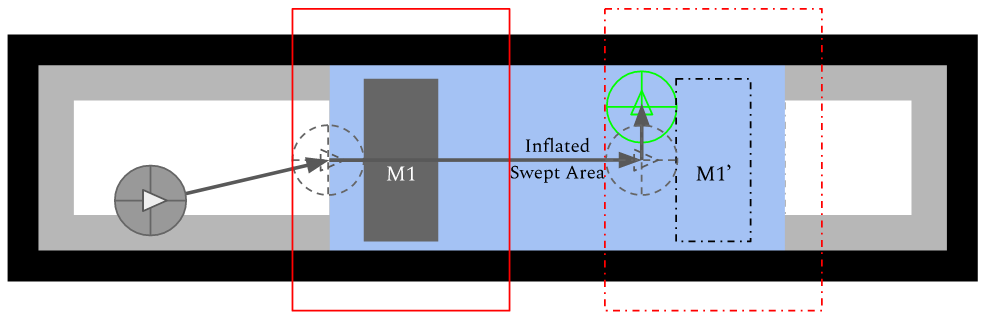
\includegraphics[width=\linewidth]{Figures/Check_New_Opening/corridor_swept.png}
  \caption{"Corridor" case}
  \label{fig:corridor_swept}
\end{subfigure}%
\begin{subfigure}{.5\textwidth}
  \centering
  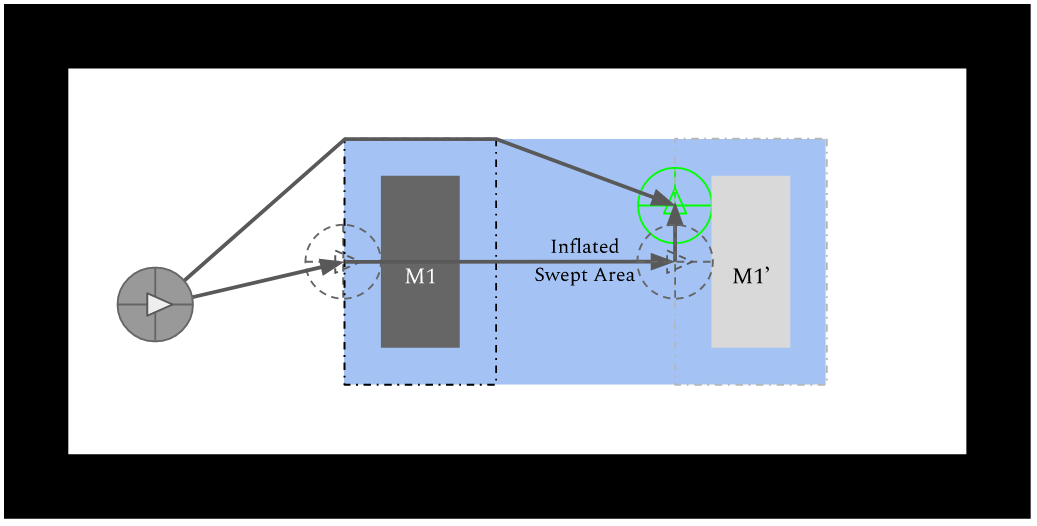
\includegraphics[width=\linewidth]{Figures/Check_New_Opening/openspace_swept.png}
  \caption{"Open space" case}
  \label{fig:openspace_swept}
\end{subfigure}
\caption{Limit cases of the original algorithm with illustration of the "Inflated swept area"}
\label{fig:inflated_swept_area}
\end{figure}

\paragraph{} In both cases, it is only interesting to consider the manipulation if it actually creates any chance of finding a path that has a lower cost than the one that avoids the obstacle. If no new opening is detected, and if, like in the "corridor" case, no path avoiding the obstacle was found, or, like in the "open space" case, a path avoiding the obstacle was found, we should only consider the manipulation if it allows us to push the obstacle through the goal pose; in more precise terms, \textbf{if the goal pose is within the "inflated swept area" and the obstacle in its final position does not intersect with the goal pose}. The inflated swept area is defined as the area covered by the inflated (by the robot's radius) obstacle when moved. In the end, the overall check condition should be:

\paragraph{} \textbf{If} CHECK-NEW-OPENING($I.occGrid$, $o$, $translation$, $BA$) AND $goalPose \in$ GET-INFLATED-SWEPT-AREA($o$, $translation$, $I$) AND $goalPose \not\in o.inflatedArea$

\paragraph{} We have an intuition that these two extra verifications steps are sufficient to restore optimality, but this is no proper demonstration. Since performance is not the main focus of our work here, but optimality is, we will prefer not to use the opening check optimization step in our following algorithms propositions, and postpone a proof to later work.

\paragraph{Note on \textbf{continue}}\label{continue_note} The \textbf{continue} statement returns the control to the beginning of the loop, and simply won't execute any of the remaining statements in the current iteration of the loop. This is done because a plan with a manipulation cannot exist without an empty $c_{1}$ component (i.e. the targeted push pose is not accessible).

\paragraph{Note on COPY}\label{copy_note} Here, $p_{opt}.o$ is a copy of object $o$, and not the same object, so that when $o$ is updated because of the call to UPDATE-FROM-NEW-INFORMATION() on $I$, we can compare the difference between the two. We do the same for $p_{opt}.pushPose$ for the same reason. This allows us to trigger re-evaluation if the obstacle's push poses change and the one the robot aimed for no longer exists.

\paragraph{Note on [] and $\neq$}\label{operators_note} Here, the [] operator is used as a short handle for "get the obstacle that corresponds in $\mathcal{O}$ that corresponds to the saved obstacle $p_{opt}.o$. The $\neq$ operator checks if the two states of the obstacle are the same or not (i.e, if the obstacle changed).

\paragraph{Note on the use of $\bigcap$}\label{area_intersect_note} The notation $\bigcap$ means here that we check for possible collisions between the swept area and any obstacle, since they may have changed.

\paragraph{Note on saving $translation$ in $p_{opt}$}\label{translation_note} The $translation$ necessary for manipulating the obstacle is saved to easily recompute the safe swept area when the obstacle changes.

\section{Social awareness through manipulation authorization consideration}\label{social_authorization_section}

\paragraph{Note on the pseudocode} The pseudocode discussed in this section and all following sections is based off the one in the first section of this chapter. For each proposition, we only modify the appropriate lines to properly highlight the indivual differences. In the last section, we merge all the propositions to give a global view of the proposed changes. The pseudocode formulation \ref{appendix_observation_section} for this proposition is available in Appendix \ref{algorithms}.

\paragraph{} As shown in Chapter \ref{Chapter2}, to the best of our knowledge, the current NAMO litterature has never covered the idea of socially-aware navigation. Then, we must ask: what makes the action of moving an obstacle socially-aware or not?

\paragraph{} The first thing that comes to mind would be to consider that some objects are better not be moved because:

\begin{itemize}
  \item they are too fragile (e.g. flower pot),
  \item they have a high value in the human’s eye (e.g. a costly vase)
  \item they might cause the robot to break if it fails to move them properly (i.e. heavy or unstable objects)
  \item they are not supposed to be moved (i.e. exhibited objects)
  \item \dots
\end{itemize}

\paragraph{} Thus comes the notion of risk, either to the robot or to the manipulated objects. To mitigate this risk, we propose to modify our base algorithm presented in the first section of this chapter, so that an obstacle is not to be moved unless identified as belonging to a provided whitelist of "movable" obstacles.

% TODO Add a link to research by Christian Wolf on object detection (go to Lyontech website to find it) or paper that justifies that detecting the nature of objects is done best by computer vision.

% TODO Add handmade figure that shows cases where Pepper might detect an obstacle or not

% TODO Add screenshots and figures of obstacle detection from video of Lyontech team to show that obstacle is not necessarily identified at the same time as it is detected

\paragraph{} This identification of the obstacle's nature is supposed to be done through computer vision, since it is one of the most efficient and most common ways to detect specific objects, by using trained neural networks for example. However, robots come with all sort of sensors to detect obstacles: laser range finders, RGB(D) cameras, sonars, ... And often, as with Pepper, their fields of vision do not perfectly overlap: typically, an obstacle may be detected by the laser range finders or the sonars, but not be within the field of vision of the RGB(D) camera, because it is in its blind spot or simply too close or too far away. This creates a situation where the robot knows an obstacle is there, but cannot definitely categorize it as "movable" or "unmovable" since it is not in the camera's field of vision.

\paragraph{} Then, it means that the algorithm must be adapted not only to manage the fact that an object should be considered for manipulation if and only if it is not deemed "unmovable", but also to eventually adapt the robot's trajectory \textbf{in an optimal way} so that an "unidentified" / "potentially movable" object can be identified with certainty before engaging with the manipulation procedure.

\paragraph{} For that, when we evaluate an obstacle, we first check whether the obstacle has already been identified or not. If it has been identified as "movable", the algorithm does not change. If it has been identified as "unmovable", the obstacle evaluation routine simply stops before actually evaluating. And finally, if the evaluated obstacle is "unidentified":

% TODO add 2D figure representing the robot and the shape of its field of vision with the appropriate parameters

% TODO add figure representing why its more interesting to choose an observation point that is closest to the robot

\begin{itemize}
  \item The $c_{1}$ plan component that goes from the current robot pose to the push pose is evaluated just as before,
  \item If a pose comprised in the computed $c_{1}$ component allows the camera field of vision to encompass the obstacle's currently known geometry, keep the precomputed $c_{1}$ component,
  \item Else we must find a shortest path component $c_{0}$ from the current robot pose to an "observation pose" where we know we can identify the obstacle as "movable" or "unmovable" with certainty and recompute $c_{1}$ as the path from this "observation pose" to the push pose. Recomputing is done in the COMPUTE-C0-C1 method, which is a baseline, naive implementation where we iterate over every "observation pose" to compute a path for $c_{0}$ and $c_{1}$ and only keep the shortest total path. Since the robot's obstacle representation may change as the robot approaches it, the condition favors paths combinations with an observation point that is closest to the current robot's pose, so that there are more chances for the robot to still have a valid observation pose in the current plan avoiding the need to recompute a plan in some cases.
  \item The observation poses are updated in the same way that push poses are: automatically, whenever an obstacle is updated. These poses are situated at every grid point for which the field of vision of the robot sensor(s) dedicated to obstacle recognition covers the entire known obstacle's geometry. Though the presented algorithm is not affected by the representation of the identification sensor's field of vision, in our experimentation, we will consider a single RGB(D) camera, and approximate its field of vision by the difference between a circular sector and a disk of same center, coincident with the robot's center, which is an acceptable representation for the Pepper robot capabilities. The circular sector has a radius $r_{max}$, central angle $\theta$ and is equally partitioned around the robot's orientation direction line. The disk has a radius $r_{min}$.
\end{itemize}

\paragraph{} In order to keep our local optimality property, we also modified the main execution loop, see Algorithm \ref{alg:04-custom-observation-makeandexecuteplan}. Basically, we added a check after the robot gets the next step to be executed and its parent plan component: if the currently considered optimal plan implies moving an obstacle that hasn't been identified yet, the next step component is $c_{0}$ or $c_{1}$, and the obstacle has changed since the previous environment observation in a way that the current plan does not allow to identify it anymore, then we must not execute the next step but re-evalutate the plan, since it may no longer be optimal.

\paragraph{Optimized version} It is obvious that the COMPUTE-C0-C1 method can be optimized in terms of execution time, in an analogous way the original algorithm did, by reducing calls to A*. A heuristic cost defined as the sum of the euclidian distance between the current pose and observation pose, and euclidean distance between observation pose and currently evaluated push pose is computed for every observation pose, and allows to order them in a list $obsPoseL$, sorted by ascending heuristic cost. The list is then traversed until the heuristic cost of the current element is greater than the current optimal cost of $c_{0}$ + $c_{1}$ allowing not to evaluate many observation points.

\paragraph{Future work} The computation and comparison if paths with observation poses may be further optimized by using a fitter algorithmic approach than calling A* as many times as needed, maybe using Dijkstra to first get the path to all observation points in a single graph search. The nature of the obstacle could also be used to adapt the way the obstacle is manipulated, for example by associating it to a specific maximum manipulation speed, which could depend on its physical characteristic.

\section{Social awareness through placement consideration}\label{social_appendix_placement_section}

\paragraph{} The pseudocode formulation \ref{appendix_placement_section} for this proposition is available in Appendix \ref{algorithms}.

\paragraph{} Now that we have achieved basic capability for the algorithm to deal with obstacles depending on whether they have been explicitly defined as "movable" or not, we have a basic answer to the question "what obstacles can be moved in a socially-aware manner?". But then, this only characterizes the obstacle itself, and not the action of moving it. When moving an obstacle, not only must we consider the obstacle we are moving, but also where we are moving it: it would definitely not be acceptable for a robot to move an obstacle in an area where it would impair other actor's movements (e.g., by blocking an entryway, a corridor, ...).

\paragraph{} Handling this, while keeping the local optimality property, can be achieved by redefining the cost of a plan not just as being dependent on the distance, time or energy, but also on the compliance to the social rule of not placing obstacles in specific places.

\paragraph{} In our proposition, we assume that "socially forbidden" areas are mapped in a similar fashion to the static obstacle map described before, with an arbitrary minimal integer value ALLOWED\_VALUE and maximal value FORBIDDEN\_VALUE. Since an obstacle may occupy several points, the total cost of moving an obstacle to some place is translated as the normalized sum of the costs of covering each point. If a point is associated with the minimal value then it means that there is no particular wish to avoid covering it with an obstacle, not affecting the total cost. On the contrary, if it is associated with the maximal value, no obstacle should ever be placed over it, raising the total cost to $+\infty$. This total cost is then simply added in the computation of the cost of the $c_{2}$ plan component as a product.

% TODO add a figure here that shows a ROS occupancy grid and its counterpart for placement consideration and add legends on colour for the text above.

\paragraph{Future work} Though we limit ourselves to a static map of "socially forbidden" areas in our implementation, nothing actually stands in the way of updating it according to the data the robot collects about the environment. This could allow to detect inappropriate areas that depend on moving or movable obstacles (e.g., behind a chair, around a wheeled table, ...). This could also, if the algorithm were also modified to handle autonomously moving objects, allow to dynamically attribute a higher placement cost in the area they are about to traverse: we would not want the robot to put an obstacle right in front of a human or a robot minding their own businesses.

\section{Taking dynamic obstacles into account}\label{dynamic_section}

\paragraph{} The pseudocode formulation \ref{appendix_dynamic_section} for this proposition is available in Appendix \ref{algorithms}.

\paragraph{} A big missing piece in the existing NAMO algorithms is that they often, as is the case with the original one we are building upon here, operate under the assumption that there are no other autonomous agents around. Therefore, an obstacle cannot move of its own volition. For the home environment setting we are aiming for, this is only acceptable if the inhabitants are not here during the robot's activities, and neither pets or other robots are. However, one of the main points of having a service robot at home is to actually interact with it. Therefore, we must at least adapt the algorithm not to enter in collision with a moving obstacle (which it would in its current state since it only invalidates a plan when \textbf{new} obstacles are found to be intersected with), and keep making locally optimal decisions.

\paragraph{} For that, it is only necessary to modify the main execution loop, since the state of the robot's knowledge about the environment only ever changes here. First thing to do is to now consider all obstacles when checking for an intersection with the current plan: $\mathcal{O}_{new}$ is no longer useful, thus removed.

\paragraph{} To keep local optimality, we chose the simplest approach: whenever an obstacle is detected as having moved, we trigger a plan re-evaluation, though we don't invalidate the current one if it is still valid (according to the same criteria as in Algorithm  \ref{alg:03-custom-basicmods-makeandexecuteplan}). For that, we assume that, when updated, the world state representation $I$ saves in a list $I.movedObstacles$ the obstacles that have moved since its last update by checking whether they don't occupy some of the space they previously occupied. If this list is not empty, then we must trigger a re-evaluation. Also, since in terms of computation time, the plan evaluation is by far the longest element, if we just went through it, then we do not directly execute the plan but go back to the beginning of the loop and check the environment again. If no obstacles moved since then, the plan will be executed. Otherwise, it will be recomputed. This way, local optimality is always guaranteed.

\paragraph{Future work} While the current proposition retains local optimality, if obstacles are constantly moving around the robot, then it will never budge, always recomputing plans, until its the environment in its field of vision stops moving. Furthermore, autonomously moving obstacles follow trajectories that can usually be predicted, at least in a short time window: it may not be interesting to invalidate the current plan and/or trigger a plan re-evaluation if an obstacle just passes by the robot in a way that would not affect the optimality of its plan. Incorporating existing work on taking obstacle trajectory predictions into account will be the object of future study. It may also be interesting to study how to merge the existing NAMO algorithms with an existing algorithm for navigation among dynamic obstacles like D* or D*Lite in a way that actually takes advantage of the incremental building of knowledge of these algorithms.

\section{Algorithm proposition}\label{merged_proposition_section}

\paragraph{} The final algorithm proposition is a merge of the previously presented individual propositions. It consists of Algorithms \ref{alg:07-custom-merge-makeandexecuteplan-part1}, \ref{alg:02-levihn-makeplan} and \ref{alg:07-custom-merge-optimized-planforobstacle-part1} and the newly created subroutines \ref{alg:04-custom-observation-optimized-compute01c1}, ref{alg:04-custom-observation-simple-checkpath} and \ref{alg:05-custom-placement-planforobstacle}. All these can be found in the Appendix \ref{algorithms}.

% Chapter 5

\chapter{Validation through simulation \& Tooling Development} % Main chapter title

\label{Chapter5} % For referencing the chapter elsewhere, use \ref{Chapter5}

\section{Portable Linux ROS Workspace for Pepper with Docker}


\section{ROS-Standards Compatible Simulator}


\section{Simulation results}

% Chapter 6

\chapter{Conclusion and Perspectives} % Main chapter title

\label{Chapter6} % For referencing the chapter elsewhere, use \ref{Chapter6}

% La conclusion n'est pas le résumé de l'écrit,  mais la fin. Elle récapitule d'abord brièvement le cheminement de pensée et en particulier les conclusions intermédiaires décrites dans le développement. Puis elle énumère les contributions/réalisations.

% La conclusion ne peut faire référence à des idées dont il n'a pas été question dans le développement. On ne saurait y trouver des faits nouveaux car la conclusion n'est en principe pas une ouverture sur d'autres idées; pour cela il est préférable d'ajouter un paragraphe "Perspectives".

% La conclusion s'ouvre plutôt sur l'action et doit être formulée très clairement, sous peine d'en diminuer l'impact.


%----------------------------------------------------------------------------------------
%	THESIS CONTENT - APPENDICES
%----------------------------------------------------------------------------------------

% \appendix % Cue to tell LaTeX that the following "chapters" are Appendices
%
% % Include the appendices of the thesis as separate files from the Appendices folder
% % Uncomment the lines as you write the Appendices
%
% \include{Appendices/AppendixA}
% %\include{Appendices/AppendixB}
% %\include{Appendices/AppendixC}

%----------------------------------------------------------------------------------------
%	BIBLIOGRAPHY
%----------------------------------------------------------------------------------------

\printbibliography[heading=bibintoc]

%----------------------------------------------------------------------------------------

\end{document}
